% vim:nojs:spelllang=en_us tw=76 sw=2 sts=2 fo+=awn fmr={-{,}-} et ts=8
\documentclass{beamer} % slides
%\documentclass[ignorenonframetext,handout]{beamer} % handout
%\documentclass{article}\usepackage{beamerarticle} % notes
%\usepackage[orientation=landscape,size=custom,width=16,height=9,scale=0.5]{beamerposter} 

%\includeonlyframes{curr1,curr2,curr3,curr4,curr5} % XXX

% Preamble							  {-{1

\mode<presentation>
{
  \usetheme{default} %Pittsburgh, default, boxes
  \setbeamertemplate{navigation symbols}{}
  \setbeamercovered{transparent}
  \setbeamersize
  {
    text margin left = 1.0em,
    text margin right = 1.0em
  }
  \setbeamercolor{section in toc}{fg=red}
  \setbeamercolor{section in toc shaded}{fg=structure}
  \setbeamertemplate{section in toc shaded}[default][100]
  %
  \setbeamerfont{bibliography entry author}{size=\tiny}
  \setbeamercolor{bibliography entry author}{fg=black}
  \setbeamercolor{bibliography entry location}{fg=black}
  \setbeamertemplate{bibliography item}{}
  \setbeamertemplate{bibliography entry title}{}
  \setbeamertemplate{bibliography entry location}{}
  \setbeamertemplate{bibliography entry note}{}
}

\usepackage[T1]{fontenc}
\usepackage[utf8]{inputenc}
\usepackage{textcomp}
\usepackage{lmodern}
\usepackage{hyperref}

\usepackage{amssymb}
\usepackage{latexsym}
\usepackage{stmaryrd}
\usepackage{extarrows}

\graphicspath{{figures/}}

\usepackage{tikz}
\usetikzlibrary{positioning,chains,matrix,shapes.arrows,scopes,
                shapes.misc,arrows,automata,calc,decorations.markings,
                decorations.text}
\everymath{\displaystyle}
\usepackage{pgf}

% Extra TikZ styles and macros {-{2

% see: 
% http://tex.stackexchange.com/questions/6135/how-to-make-beamer-overlays-with-tikz-node
\tikzset{onslide/.code args={<#1>#2}{%
  \only<#1>{\pgfkeysalso{#2}} % \pgfkeysalso doesn't change the path
}}

\tikzset{dimmedmarker/.code args={<#1> then <#2>}{%
  \alt<#1,#2>
  {
    \tikzstyle{marker} = [draw]
    \alt<#2>
    {\pgfkeysalso{->,red!80,draw opacity=.15}}
    {\pgfkeysalso{->,red!80,draw opacity=.50}}
  }
  {
    \tikzstyle{marker} = [draw=none]}
}}

\tikzset{zdimmedmarker/.code args={<#1> then <#2>}{%
  \alt<#1,#2>
  {
    \tikzstyle{marker} = [draw]
    \alt<#2>
    {\pgfkeysalso{->,blue!80,draw opacity=.15}}
    {\pgfkeysalso{->,blue!80,draw opacity=.50}}
  }
  {
    \tikzstyle{marker} = [draw=none]}
}}

\tikzstyle{every picture}+=[remember picture]
\tikzstyle{na} = [baseline=-.5ex]
\tikzstyle{ln} = [baseline,every node/.style={anchor=base,inner sep=0}]
\tikzstyle{lm} = [baseline,every node/.style={anchor=base}]

\tikzstyle{weak} =
  [decoration={markings,
               mark=at position -.6mm with {\draw[fill=white] circle (.6mm);},
               mark=at position -1.1mm with {\arrow{latex}},
              }, postaction={decorate}]

\tikzstyle{strong} =
  [decoration={markings,
               mark=at position .6mm with {\draw[fill=white] circle (.6mm);},
                  }, postaction={decorate}, -latex]

% 1 - width (e.g., .95\textwidth); 2 - image name/path
\newenvironment{hgraphicscope}[2]
  {
    \node[anchor=south west,inner sep=0] (image) at (0,0)
       {\includegraphics[width=#1]{#2}};
    \begin{scope}
    \tikzset{every node/.style={}, every path/.style={}}
    \clip (image.south west) rectangle (image.north east);
    \path let \p1=(image.south east) in (\y1, \x1) coordinate (ylimit);
    \end{scope}
    \begin{scope}[x={(image.south east)},y={(ylimit)},scale=0.1,]
  }
  {
    \end{scope}
  }

% see: 
% http://tex.stackexchange.com/questions/16357/how-can-i-position-an-image-in-an-arbitrary-position-in-beamer
% Usage:
% \tikzoverlay at (-1cm,-5cm) {content};
% or
% \tikzoverlay[text width=5cm] at (-1cm,-5cm) {content};
\tikzset{every overlay node/.style={anchor=north west}}
\def\tikzoverlay{%
   \tikz[baseline,overlay]\node[every overlay node]
}%

%---  }-}2------------------------------------------------------------

\newcommand{\ipause}{\onslide+<+(1)->}
\newcommand{\makepoint}[1]{\textcolor{structure}{\textbf{#1}}}

% Useful slide macros

\newcommand<>{\blue}[1]{{\color#2{blue}{#1}}}
\newcommand<>{\green}[1]{{\color#2{green}{#1}}}
\newcommand<>{\red}[1]{{\color#2{red}{#1}}}
\newcommand<>{\violet}[1]{{\color#2{violet}{#1}}}
\newcommand<>{\gray}[1]{{\color#2{gray}{#1}}}

\usepackage[final,formats]{listings}
%\lstset{language=<...>,basicstyle=\sffamily}

\lstdefinelanguage{hybrid}
   {morekeywords={
	let,in,rec,where,end,if,then,else,do,done,run,
	open,
	fun,node,hybrid,
	match,with,automaton,emit,
	pre,when,whenot,fby,merge,on,clock,
	or,and,not,as,mod,
	unless,until,continue,reset,every,await,
	init,der,type,last,
        period,local,present
    },
    sensitive=true,
    morecomment=[n]{(*}{*)},
    morestring=[b]",
    mathescape=true,
    basicstyle=\sffamily\footnotesize,
    literate={->}{{$\rightarrow\;$}}1
    }

\lstnewenvironment{hybrid}
    {\lstset{language=hybrid}}
    {}

%int boolean float char string
%sig static

\newcommand{\hy}[1]{\ensuremath{\mbox{\lstinline[language=hybrid]{#1}}}}
\newcommand{\hys}[1]{\ensuremath{\mbox{\lstinline[language=hybrid,basicstyle=\sffamily\tiny]{#1}}}}



%--   }-}1%%%%%%%%%%%%%%%%%%%%%%%%%%%%%%%%%%%%%%%%%%%%%%%%%%%%%%%%%%%%

\begin{document}

\pgfdeclareimage[height=1.3cm]{aircraft}{figures/a330.pdf}

\begin{frame}{Air Traffic Conflict Resolution} %{-{1

\tikzoverlay[text width=15.5em] at (6.8cm,1.9cm) {
\begin{thebibliography}{1}
\bibitem{TomlinPapSas:AirTraffic:1998}
C.~Tomlin, G.~J. Pappas, and S.~Sastry.
\newblock Conflict resolution for air traffic management: A study in multiagent
  hybrid systems.
\newblock {\em IEEE Trans. Automatic Control}, 43(4):509--521, Apr. 1998.
\end{thebibliography}
};

\begin{minipage}[T]{.52\textwidth}
\begin{tikzpicture}[scale=.85]%{-{2
  \useasboundingbox (0,0) circle (3.6cm);
  \draw
    (0,0) node[rotate=-90] {\pgfuseimage{aircraft}}
    (2.5,4.0) node[rotate=150] {\pgfuseimage{aircraft}}
    ;
  \draw[gray]
    (0,0) circle (1.5cm)
    (0,0) circle (3.7cm)
    ;
  \path [decorate,
         decoration={text along path, text={protected zone}, text color=gray},
         rotate=-135]
    (0,0) circle (1.4cm)
    ;
  \path [decorate,
         decoration={text along path, text={alert zone}, text color=gray},
         rotate=-103, gray]
    (0,0) circle (3.6cm)
    ;
  %
\end{tikzpicture}%}-}2$
\end{minipage}%
\begin{minipage}[T]{.48\textwidth}

\begin{itemize}

\item Original: calculate a \emph{maximal set of safe initial conditions for 
each aircraft} for a maneuver

\item Simulation: single initial state, deterministic

\item \blue{Focus on modeling resets in hybrid automata}

\end{itemize}

\pause
\bigskip
\medskip

\begin{itemize}

\item Two virtual cylinders around each aircraft:
  \begin{itemize}
  \item[protected zone] zones must never overlap
  \item[alert zone] must exchange information for conflict prediction and 
  resolution
  \end{itemize}

\end{itemize}

\end{minipage}%

\end{frame}
%--   }-}1%%%%%%%%%%%%%%%%%%%%%%%%%%%%%%%%%%%%%%%%%%%%%%%%%%%%%%%%%%%%

\begin{frame}{Air Traffic Conflict Resolution} %{-{1

\begin{minipage}[T]{.5\textwidth}
\begin{tikzpicture}[scale=.85]%{-{2
  \useasboundingbox (0,0) circle (3.6cm);
  \draw
    (0,0) node[rotate=-90] {\pgfuseimage{aircraft}}
    ;
  \draw[gray!20]
    (0,0) circle (1.5cm)
    (0,0) circle (3.7cm)
    ;
  \path [decorate,
         decoration={text along path, text={protected zone},
         text color=gray!20},
         rotate=-135]
    (0,0) circle (1.4cm)
    ;
  \path [decorate,
         decoration={text along path, text={alert zone},
         text color=gray!20},
         rotate=-103]
    (0,0) circle (3.6cm)
    ;
  %
  \draw[dashed, every node/.style={inner sep=1},green]
    (0,0) circle (1.9cm) +(45:1.9cm) node[above right] {$\alpha_1$}
    ;
  \draw[dashed, every node/.style={inner sep=1},violet]
    (0,0) circle (2.9cm) +(45:2.9cm) node[above right] {$\alpha_2$}
    ;
\end{tikzpicture}%}-}2$
\end{minipage}%
\begin{minipage}[T]{.5\textwidth}

\begin{description}
\item[Cruise] Cruise until aircraft are \green{$\alpha_1$} miles apart.
\item[Left]   Each aircraft changes heading by $\Delta^{\circ}$. Both fly
              until $d$ miles apart.
\item[Straight] Each returns to original heading. Both fly until
                \violet{$\alpha_2$} miles apart.
\item[Right]  Each changes heading by $-\Delta^{\circ}$ and returns
              to original flight path.
\end{description}
\end{minipage}%

\end{frame}
%--   }-}1%%%%%%%%%%%%%%%%%%%%%%%%%%%%%%%%%%%%%%%%%%%%%%%%%%%%%%%%%%%%

\begin{frame}{Air Traffic Conflict Resolution} % {-{1

\centering
\begin{tikzpicture}[scale=.85]%{-{2
  \begin{scope} %{-{3
    \draw[dashed,->]
      (-1,0) coordinate (airc1)
      -- ++(3.5,0) coordinate (aircang)
      -- ++(45:1)
      -- ++(1,0) coordinate (aircd)
      -- ++(1,0)
      -- ++(-45:1)
      -- ++(1,0)
      ;
    \draw[gray]
      (aircang) -- +(1.0,0)
      +(0.8,0) [scale=.8]arc (0:45:1.0)
      +(1.4,-.2) node {\tiny$\Delta\phi$}
      (aircd) -- (aircd |- airc1)
      node[above right] {\tiny$d$}
      ;
    \draw
      (airc1) node[rotate=-90] {\pgfuseimage{aircraft}}
      ;
  \end{scope} %}-}3
  \begin{scope}[rotate=90] %{-{3
    \draw[dashed,->,font=\small]
      (-3.8,-2) coordinate (airc1)
      -- node[left] {cruise} ++(2.5,0) coordinate (aircang)
      -- node[below left] {left} ++(45:1)
      -- ++(1,0) coordinate (aircd)
      -- node[left] {straight} ++(1,0)
      -- node[above left] {right} ++(-45:1)
      -- node[right] {cruise} ++(1,0)
      ;
    \draw[gray]
      (aircang) -- +(1.0,0)
      +(0.8,0) [scale=.8]arc (0:45:1.0)
      +(.3,-0.8) node {\tiny$\Delta\phi$}
      (aircd) -- (aircd |- airc1)
      node[above left] {\tiny$d$}
      ;
    \draw
      (airc1) node[rotate=0] {\pgfuseimage{aircraft}}
      ;
  \end{scope} %}-}3
  %
  \node at (-.7,-4) {\tiny{\emph{(Fig. 2, Tomlin et al.)}}};
  %
  \node[below right,scale=1.176] at (2.5,-1.0) {
      \begin{minipage}{6.9cm}
        \begin{itemize}

        \item The maneuver looks like this from a fixed perspective

        \item But the model is relative to aircraft 1: only aircraft 2 
        appears to move

        \item Note also that heading changes are modeled as instantaneous 
        and simultaneous

        \end{itemize}
      \end{minipage}
  };
\end{tikzpicture}%}-}2$
\end{frame}

%--   }-}1%%%%%%%%%%%%%%%%%%%%%%%%%%%%%%%%%%%%%%%%%%%%%%%%%%%%%%%%%%%%

\begin{frame}{Air Traffic Conflict Resolution} % {-{1

\centering
\scalebox{.7}{
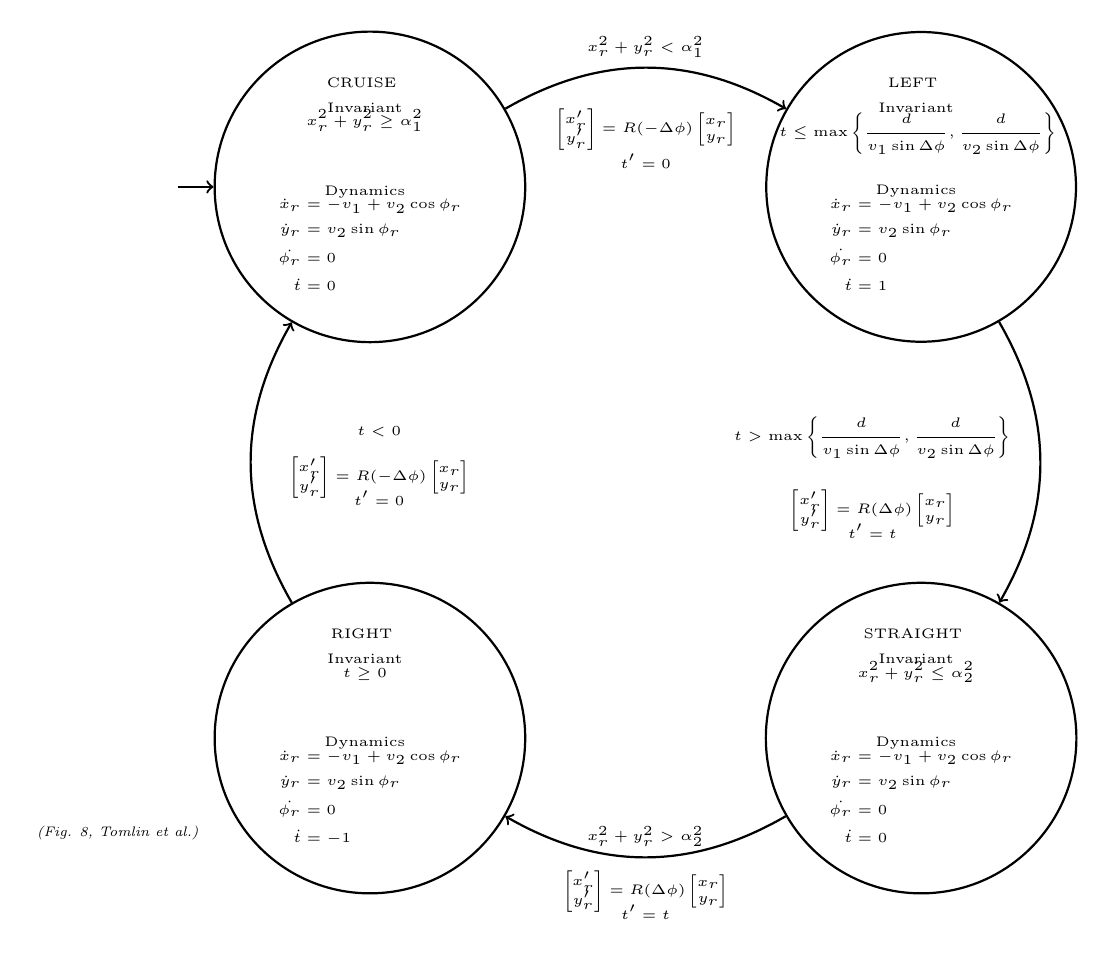
\begin{tikzpicture}[
    ->,
    thick,
    auto,
    node distance=7.0cm,
    initial text=,
    font=\tiny
]

   \node[state,initial] (Cruise)
     {\begin{minipage}{2.2cm}\centering %{-{2
         CRUISE
         \smallskip

         Invariant
         \vskip-2.5em
         \[x_r^2 + y_r^2 \geq \alpha_1^2\]
         \smallskip

         Dynamics
         \vskip-2.5em
         \begin{align*}
           \dot{x}_r    &= -v_1 + v_2\cos\phi_r\\
           \dot{y}_r    &= v_2\sin\phi_r\\
           \dot{\phi_r} &= 0\\
           \dot{t}      &= 0
         \end{align*}
       \end{minipage}}; %}-}2

   \node[state] (Left) [right of=Cruise]
     {\begin{minipage}{2.2cm}\centering %{-{2
         LEFT
         \smallskip

         Invariant
         \vskip-2.5em
         \[\ \ \ \ \llap{$t\leq\max$}\left\{\frac{d}{v_1\sin\Delta\phi},
         \frac{d}{v_2\sin\Delta\phi}\right\}\]

         Dynamics
         \vskip-2.5em
         \begin{align*}
           \dot{x}_r    &= -v_1 + v_2\cos\phi_r\\
           \dot{y}_r    &= v_2\sin\phi_r\\
           \dot{\phi_r} &= 0\\
           \dot{t}      &= 1
         \end{align*}
       \end{minipage}}; %}-}2

   \node[state] (Straight) [below of=Left]
     {\begin{minipage}{2.2cm}\centering %{-{2
         STRAIGHT
         \smallskip

         Invariant
         \vskip-2.5em
         \[x_r^2 + y_r^2 \leq \alpha_2^2\]
         \smallskip

         Dynamics
         \vskip-2.5em
         \begin{align*}
           \dot{x}_r    &= -v_1 + v_2\cos\phi_r\\
           \dot{y}_r    &= v_2\sin\phi_r\\
           \dot{\phi_r} &= 0\\
           \dot{t}      &= 0
         \end{align*}
       \end{minipage}}; %}-}2

   \node[state] (Right) [below of=Cruise]
       {\begin{minipage}{2.2cm}\centering % {-{2
         RIGHT
         \smallskip

         Invariant
         \vskip-2.5em
         \[t \geq 0\]
         \smallskip

         Dynamics
         \vskip-2.5em
         \begin{align*}
           \dot{x}_r    &= -v_1 + v_2\cos\phi_r\\
           \dot{y}_r    &= v_2\sin\phi_r\\
           \dot{\phi_r} &= 0\\
           \dot{t}      &= -1
         \end{align*}
       \end{minipage}}; %}-}2

   \path (Cruise) edge [bend left]
      node[above] {$x_r^2 + y_r^2 < \alpha_1^2$}
      node[below]
          {\begin{minipage}{3cm} %{-{2
              \[
                \begin{bmatrix} x_r'\\ y_r' \end{bmatrix}
                =
                R(-\Delta\phi)
                \begin{bmatrix} x_r\\ y_r \end{bmatrix}
              \]
              \vskip-1.5em
              \[
                t' = 0
              \]
           \end{minipage}} %}-}2
      (Left);

   \path (Left) edge [bend left]
       node[left]
          {\begin{minipage}{4cm} %{-{2
               \[t>\max\left\{\frac{d}{v_1\sin\Delta\phi},
                 \frac{d}{v_2\sin\Delta\phi}\right\}\]
              \[
                \begin{bmatrix} x_r'\\ y_r' \end{bmatrix}
                =
                R(\Delta\phi)
                \begin{bmatrix} x_r\\ y_r \end{bmatrix}
              \]
              \vskip-1.5em
              \[
                t' = t
              \]
           \end{minipage}} %}-}2
      (Straight);

   \path (Straight) edge [bend left]
      node[above] {$x_r^2 + y_r^2 > \alpha_2^2$}
      node[below]
          {\begin{minipage}{4cm} %{-{2
              \[
                \begin{bmatrix} x_r'\\ y_r' \end{bmatrix}
                =
                R(\Delta\phi)
                \begin{bmatrix} x_r\\ y_r \end{bmatrix}
              \]
              \vskip-1.5em
              \[
                t' = t
              \]
           \end{minipage}} %}-}2
      (Right);

   \path (Right) edge [bend left]
      node[right]
          {\begin{minipage}{3cm} %{-{2
              \[t < 0\]
              \[
                \begin{bmatrix} x_r'\\ y_r' \end{bmatrix}
                =
                R(-\Delta\phi)
                \begin{bmatrix} x_r\\ y_r \end{bmatrix}
              \]
              \vskip-1.5em
              \[
                t' = 0
              \]
           \end{minipage}} %}-}2
      (Cruise);

  \node at (-3.2,-8.2) {\tiny{\emph{(Fig. 8, Tomlin et al.)}}};
\end{tikzpicture}}%}}}4

\end{frame}

%--   }-}1%%%%%%%%%%%%%%%%%%%%%%%%%%%%%%%%%%%%%%%%%%%%%%%%%%%%%%%%%%%%

\end{document}
